\section{Box-Jenkins analysis} 

Before going further and select a model that will be able to predict the air temperature in Recife for the months following the year $1995$, we need to detrend and deseasonalize our time serie. 

% TODO: explain why we need stationary time series

\subsection[short]{Differencing}

We first remove the seasonality by taking a seasonal difference which consist by taking the difference between an observation and the previous observation at the same season (in our case, $12$ months before): $X'_t = X_t - X_{t-12}$. 
Then, we remove the trend by first differencing the serie.

\begin{figure}[H]
	\centering
	\begin{subfigure}{0.49\textwidth}
		\centering
		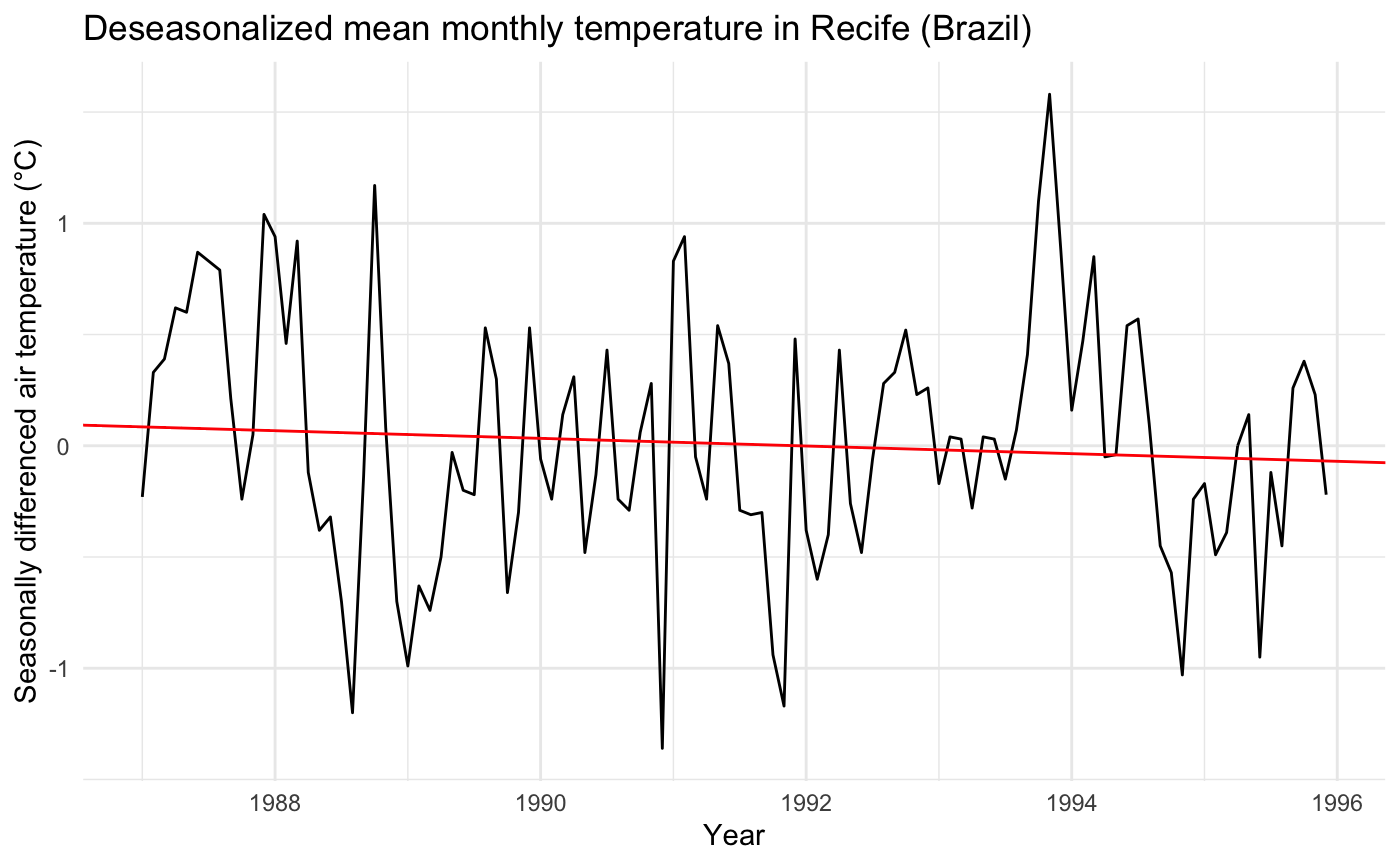
\includegraphics[width=\textwidth]{figures/box_jenkins/deseasonalized_time_serie.png}
		\label{fig:deseasonalized-time-serie}
	\end{subfigure}
	\begin{subfigure}{0.49\textwidth}
		\centering
		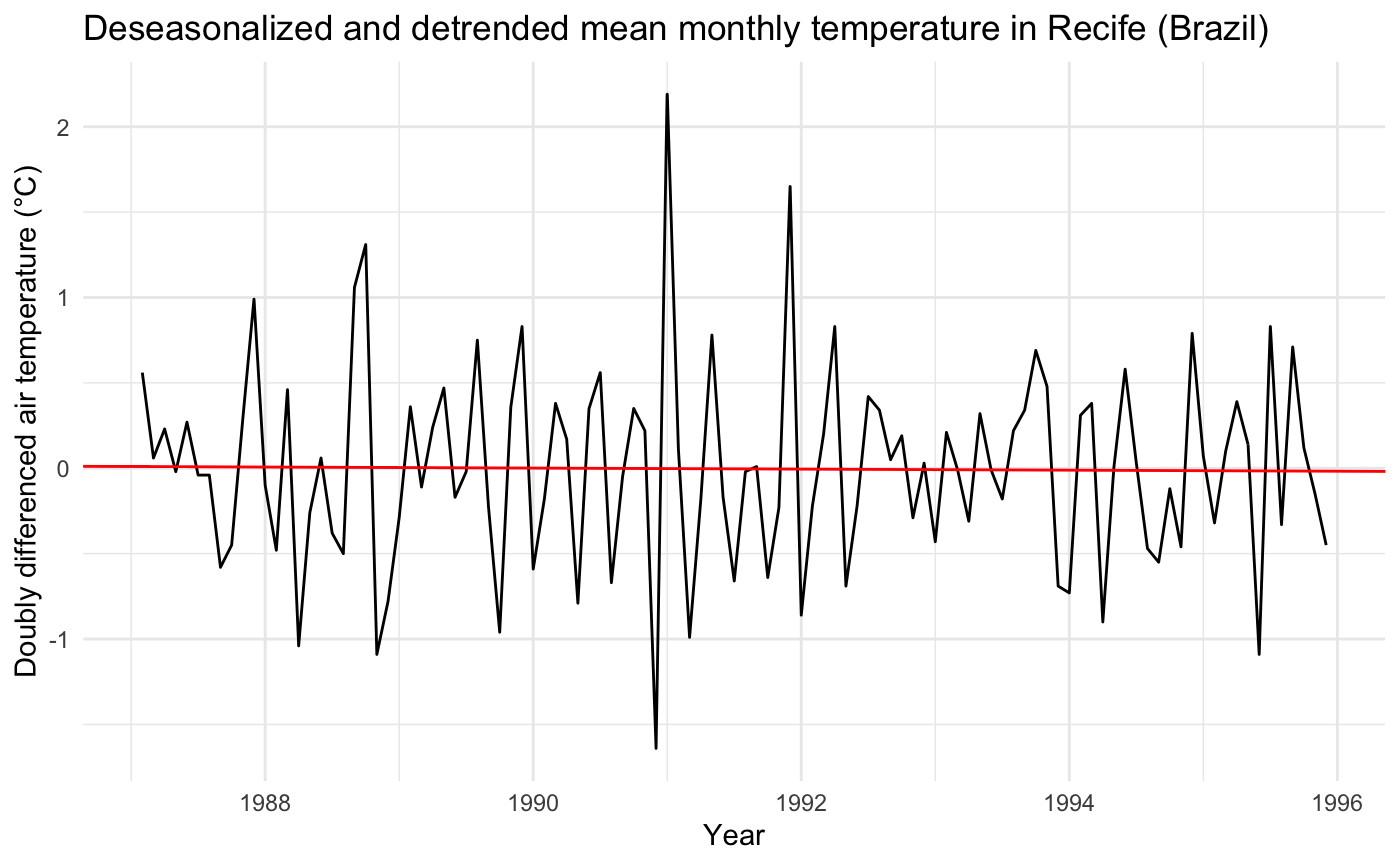
\includegraphics[width=\textwidth]{figures/box_jenkins/doubly_differenced_time_serie.png}
		\label{fig:doubly-differenced-time-serie}
	\end{subfigure}
	\caption{Deseasonalized time serie (at left) and doubly differenced time serie (deseasoned and detrended) (at right). In red is the regression line.}
\end{figure}

After doubly differencing, the time serie is now stationary as shown on the plots above.

\subsection{Model intuition with ACF and PACF plots}

We can now look at the ACF and PACF plots.

\subsection{Automatic model selection with AIC and BIC}